\chapter[Materiais Compostos]{Materiais Compostos}

\section{Desenvolvimento histórico}
A implementação do uso de materiais compostos na indústria aeronáutica civil e militar seguiu os estágios típicos da implementação de qualquer nova tecnologia no mercado. Segundo \cite{kassapoglou2013design}, primeiramente o uso da tecnologia de materiais compostos foi limitado às estruturas secundárias visto que minimizavam os riscos envolvidos e também possibilitava a coleta de dados, o que viabilizava uma melhor compreensão do comportamento das estruturas que possuiam essa tecnologia.

De acordo com \cite{daniel2006engineering}, em 1942 o primeiro barco constiuído de fibra de vidro foi fabricado, e nos anos 1950 as primeiras aplicações com materiais compostos em mísseis foram realizadas. Referindo-se a indústria aeronáutica no último século, o primeiro uso de materiais compostos mais avançados, segundo \cite{kassapoglou2013design}, ocorreu no final da década de 1950 na aeronave \emph{Akaflieg Phonix FS-24}. Essa aeronave consistiu em um planador projetado por professores e alunos da Universidade de Stuttgart e foi construído, inicialmente de madeira balsa, e posteriormente teve sua estrutura alterada para um sanduíche de compósitos de fibra de vidro com madeira tipo balsa. Após isso, no fim dos anos 1960, com a nova geração de materiais compostos avançados, como o carbono, a indústria de helicópteros foi a primeira a utilizá-los em estruturas primárias, destacando o projeto do \emph{Aerospatiale AS-341 Gazelle}. Este helicóptero foi considerado um dos mais modernos na época, não só porque ele possuía um inovador rotor de cauda reduzindo drasticamente a emissão de ruídos, mas também, pelo fato de as pás do rotor principal serem constituídas de material composto.

Por volta dos anos 1970 as primeiras aeronaves majoritariamente constituídas de materiais compostos começaram a surgir. Essas aeronaves eram pequenas e normalmente para uso recreativo ou para acrobacias, visto que com o uso de materiais compostos era possível obter uma redução de peso estrutural e portanto, aeronaves mais rápidas e ágeis quando comparadas às aeronaves da época. O uso de material composto teve início em aeronaves pequenas também pelo fato de os requisitos de certificação estrutural para aeronaves menores serem mais facilmente cumpridos quando comparados aod requisitos das aeronaves de grande porte. Além disso, de acordo com \cite{kassapoglou2013design}, a performance dos materias compostos não era completamente conhecida, por exemplo, a sensitividade desse tipo de material ao dano por impacto e suas implicações para o projeto só foram ser melhor conhecidas no final dos anos 1970. Portanto, somente no final dos anos 1970 e início dos anos 1980 que a utilização de materiais compostos começou a ser expandida para aeronaves de porte maior, como a concepção da empenagem horizontal do \emph{Boeing 737}, que era uma estrutura primária construída de um sanduíche de materias compostos. Seguindo a aplicação em grande escala de materiais compostos, destaca-se o \emph{Airbus A320}, no qual tanto a empenagem horizontal e a vertical, quanto as superfícies de controle foram projetadas e fabricadas utilizando material composto.

A proxíma aplicação significante desse tipo de material em estruturas primárias foi no início dos anos 1990 com o \emph{Boeing 777}, em que além das empenagens e superfícies de controle, as vigas principais do piso eram constituídas de material composto.
Segundo \cite{daniel2006engineering}, o maior sinal de aceitação do uso de materiais compostos na indústria aeronáutica civil, ocorreu no \emph{Boeing 787 Dreamliner}, em que materiais como carbono/\emph{epoxy} e grafite/titânio constituíam cerca de 50\% do peso da aeronave, incluindo majoritariamente asas e fuselagem. Destaca-se também o \emph{Airbus A380}, que utiliza materiais compostos, incluindo o \emph{GLARE}, um laminado híbrido de fibra de vidro/\emph{epoxy}/alumínio, que combina as vantagens e desvantagens dos materiais metálicos e compostos.

Observa-se, portanto, que o uso dos materiais compostos vem aumentando de maneira significativa na indústria aeronáutica. Uma maneira de perceber o aumento do uso de materiais compostos nessa indústria é com base na \autoref{fig_usecomposites}, em que fica claro o aumento percentual da utilização desse tipo de material em relação ao peso das estruturas de vários modelos de aeronaves.

\begin{figure}[h]
	\caption{\label{fig_usecomposites}Uso de materiais compostos na indústria aeronáutica.}
  \centering
  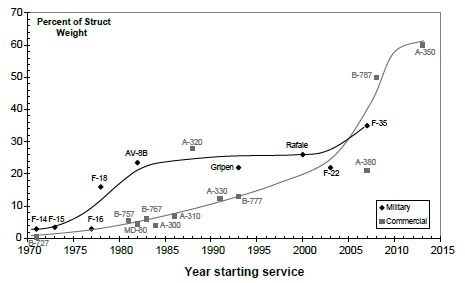
\includegraphics[scale=1.1]{figura/UseOfComposites}
	\legend{Fonte: \cite[p. 6]{kassapoglou2013design}}
\end{figure}

\section{Visão geral}
De acordo com \cite{daniel2006engineering}, os materiais compostos possuem diversas vantagens de utilização em relação aos materiais metálicos como a elevada resistência, a elevada rigidez, a vida longa em fadiga, a baixa densidade e a alta adaptabilidade em relação a função de utilização pretendida pela estrutura. A superior perfomance estrutural dos materiais compostos se deve basicamente às elevadas resistência e rigidez específicas e à anisotropia do material, visto que devido à esta última característica, o material composto possui diversos graus de liberdade para uma configuração ótima do laminado. No geral, devido ao elevado número de graus de liberdade é possível realizar a otimização do laminado em material composto para diversas restrições de projeto e objetivos, como menor peso estrutural, máxima estabilidade dinâminca e/ou menor custo de fabricação. No entanto, todo o processo requer um confiável banco de dados das propriedades dos materiais, métodos de análises estruturais, técnicas de modelagem e simulações padronizadas e certificadas. Logo, devido às numerosas opções disponíveis, os processos e análises acabam se tornando mais complexos e custos em relação aos dos materiais convencionais.

Os materiais compostos possuem algumas limitações de uso em relação ao materiais metálicos. Do ponto de vista da micromecânica, as fibras dos materiais compostos possuem uma grande variabilidade nas propriedades de resistência e concentradores de tensão locais reduzem consideravelmente a resistência a tração das estruturas projetadas em materiais compostos. Em relação a macromecânica, a anisotropia do material pode ser utilizada considerada como uma vantagem visto que o comportamento do material pode ser variado, no entando, esta mesma característica faz com que as análises desses materiais sejam muito mais complexas \cite{daniel2006engineering}.

\section{Teoria Clássica da Laminação}
De acordo com \cite{daniel2006engineering} para o desenvolvimento da Teoria Clássica da Laminação, assumem-se as seguintes premissas e restrições:
\begin{enumerate}
  \item Cada lâmina do laminado é quasi-homogênea e ortotrópica;
	\item O laminado é fino com as suas dimensões laterais muito maiores do que a sua espessura e é carregado somente no plano, isto é, o lamninado e suas lâminas (exceto as bordas) estão em um estado plano de tensão ($\sigma_z = \tau_{xz} = \tau_{yz} =  $ 0);
	\item Todos os deslocamentos são pequenos comparados com a espessura do laminado ($|u|,|v|,|w| \ll h$);
	\item Deslocamentos são contínuos ao longo da espessura;
	\item Deslocamentos no plano variam linearmente ao longo da espessura do laminado, isto é, os deslocamentos $\emph u$ e $\emph v$ nas direções $\emph x$ e $\emph y$ são funções lineares de $\emph z$;
	\item Linhas retas normais à superfície média permanece reta e normal à essa superfície após a deformação. Isto implica que as deformações transversais de cisalhamento $\gamma_{xz}$ e $\gamma_{yz}$ são nulas;
	\item As relações deformações-deslocamentos e tensões-deformações são lineares;
	\item Distâncias normais à superfície média permanecem constantes, isto é, o deslocamento transversal normal, $\varepsilon_{z}$ é zero. Isto implica que o deslocamento transversal $\emph w$ é independente da coordenada de espessura $\emph z$.
\end{enumerate}

\subsection{Relações entre deformações e deslocamentos}
Seguindo a \autoref{fig_laminatedeformation} como referência, tem-se que o plano $\emph x-y$ é o plano médio do laminado, ou seja, é equidistante do laminado mais superior e do mais inferior. Portanto, este plano é chamado de \emph{Plano médio} ou \emph{Plano de referência}.

\begin{figure}[h]
	\caption{\label{fig_laminatedeformation}Seção do laminado antes (ABCD) e depois da deformação (A'B'C'D').}
  \centering
  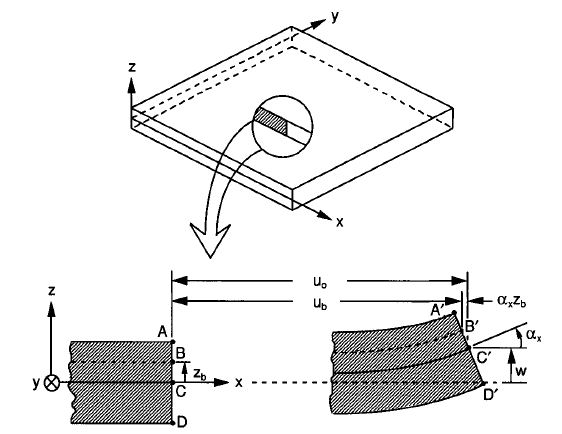
\includegraphics[scale=1.0]{figura/LaminateDeformation}
	\legend{Fonte: \cite{daniel2006engineering}}
\end{figure}

Tem-se que os deslocamentos no plano $u_0$ e $v_0$ nas direções $\emph x$ e $\emph y$ e o deslocamento fora do plano $w$ na direção $\emph z$ são funções somente de x e y, como mostrado a seguir.
\begin{equation} \label{displacements}
\begin{split}
u_{o}=u_{o}(x,y)\\
v_{o}=v_{o}(x,y)\\
w=f(x,y)
\end{split}
\end{equation}
E que as rotações ao longo dos eixos x e y são dadas por:
\begin{equation} \label{rotations}
\begin{split}
\alpha_{x}=\dfrac{\partial w} {\partial x}\\
\alpha_{y}=\dfrac{\partial w} {\partial y}
\end{split}
\end{equation}

Portanto, os componentes de deslocamentos de um ponto $B$ de coordenada $z_b$, onde z é a coordenada na espessura do laminado, são:
\begin{equation} \label{displacements_B}
\begin{split}
u=u_{o} - \dfrac{\partial w}{\partial x}\\
v=v_{o} - \dfrac{\partial w}{\partial y}
\end{split}
\end{equation}

Para pequenos deslocamentos, as relações clássicas de deformação e deslocamento no campo elástico são dadas por:
\begin{equation} \label{Strain_Displacement}
\begin{gathered}
\varepsilon_{x} = \dfrac{\partial u}{\partial x} = \dfrac{\partial u_o}{\partial x} - z\dfrac{\partial^2 w}{\partial x^2}\\~\\
\varepsilon_{y} = \dfrac{\partial v}{\partial y} = \dfrac{\partial v_o}{\partial y} - z\dfrac{\partial^2 w}{\partial y^2}\\~\\
\gamma_{xy} = \gamma_z = \dfrac{\partial u}{\partial y} + \dfrac{\partial v}{\partial x} = \dfrac{\partial u_o}{\partial y} + \dfrac{\partial v_o}{\partial x} - 2z\dfrac{\partial^2 w}{\partial x\partial y}
\end{gathered}
\end{equation}

Sabe-se ainda, por definição, que:
\begin{equation} \label{Strain_Curvatures}
\begin{gathered}
\varepsilon^o_{x} = \dfrac{\partial u_o}{\partial x}\\~\\
\varepsilon^o_{y} = \dfrac{\partial v_o}{\partial y}\\~\\
\gamma^o_{xy} = \gamma^o_z= \dfrac{\partial u_o}{\partial y} + \dfrac{\partial v_o}{\partial x}\\~\\
\kappa_x = -\dfrac{\partial^2 w}{\partial x^2}\\~\\
\kappa_y = -\dfrac{\partial^2 w}{\partial y^2}\\~\\
\kappa_{xy} = \kappa_z = -2\dfrac{\partial^2 w}{\partial x\partial y}
\end{gathered}
\end{equation}

Portanto, as deformações em qualquer ponto do laminado podem ser relacionadas às deformações do plano e às curvaturas do laminado como mostrado a seguir:

\begin{equation} \label{matrix_strain}
\begin{bmatrix}
    \varepsilon_{x} \\
    \varepsilon_{y} \\
    \gamma_{z} \\
\end{bmatrix}
=
\begin{bmatrix}
		\varepsilon^o_{x} \\
		\varepsilon^o_{y} \\
		\gamma^o_{z} \\
\end{bmatrix}
+z
\begin{bmatrix}
    \kappa_{x} \\
    \kappa_{y} \\
    \kappa_{z} \\
\end{bmatrix}
\end{equation}

\subsection{Relações entre tensões e deformações de uma lâmina dentro de um laminado}
Considera uma lâmina específica, \emph{k} em um laminado multidirecional, na qual a distância \emph{$z_k$} se refere a distância da lâmina ao plano de referência do Laminado. Tem-se que as relações de tensão-deformação para essa lâmina, no sistema de coordenada do laminado valem:

\begin{equation} \label{matrix_stress_strain}
\begin{bmatrix}
    \sigma_{x} \\
    \sigma_{y} \\
    \tau_{s} \\
\end{bmatrix}_k
=
\begin{bmatrix}
		Q_{xx} & Q_{xy} & Q_{xs} \\
		Q_{yx} & Q_{yy} & Q_{ys} \\
		Q_{sx} & Q_{sy} & Q_{ss} \\
\end{bmatrix}_k
\begin{bmatrix}
    \varepsilon_{x} \\
    \varepsilon_{y} \\
    \gamma_{s} \\
\end{bmatrix}_k
\end{equation}

Em que a rigidez representada por $Q$, vale:
\begin{equation} \label{StiffnessQ}
\begin{gathered}
Q_{xx} = E_{11} - \dfrac{E^2_{13}}{E_{33}}\\~\\
Q_{xy} = E_{12} - \dfrac{E_{13}E_{23}}{E_{33}}\\~\\
Q_{yy} = E_{22} - \dfrac{E^2_{23}}{E_{33}}\\~\\
Q_{xs} = E_{66}
\end{gathered}
\end{equation}
Onde $E_{11}, E_{12}, E_{13}, E_{22}, E_{23}, E_{33}$ e $E_{66}$ são constantes elásticas independentes do material.

Substituindo a \autoref{matrix_strain} na \autoref{matrix_stress_strain} tem-se, de forma generalizada, a seguinte expressão para as deformações:

\begin{equation} \label{general_stress_strain}
		[\sigma]^k_{x,y}=[Q]^k_{x,y}[\varepsilon^o]_{x,y}+z[Q]^k_{x,y}[\kappa]_{x,y}
\end{equation}

Nota-se, portanto, das \autoref{matrix_strain} e \autoref{general_stress_strain} que mesmo que as deformações variem linearmente, não necessariamente as tensões variam da mesma maneira. Devido à discontinuidade da matriz de rigidez $[Q]_{x,y}$ ao longo das lâminas do laminado, as tensões também podem variar de forma discontínua ao longo das lâminas.

\subsection{Relações envolvendo forças e momentos resultantes}
Tendo como referência a \autoref{fig_laminateforces} e sabendo que as tensões ao longo do laminado variam devido às diferentes matrizes de rigidez de cada lâmina específica, pode-se fazer uma integração para obter forças e momentos resultantes.

\begin{figure}[h]
	\caption{\label{fig_laminateforces}Elemento de uma lâmina com forças e momentos resultantes.}
  \centering
  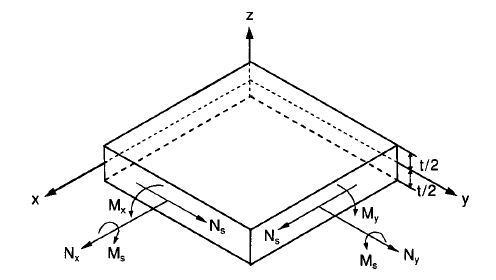
\includegraphics[scale=1.0]{figura/LaminateForcesMoments}
	\legend{Fonte: \cite{daniel2006engineering}}
\end{figure}

As expressões seguintes se relacionam a essas forças e momentos resultantes.

\begin{equation} \label{ForcesMoments}
\begin{gathered}
N^k_{x}=\int^{t/2}_{-t/2}\sigma_x\emph{dz}\\~\\
N^k_{y}=\int^{t/2}_{-t/2}\sigma_y\emph{dz}\\~\\
N^k_{s}=\int^{t/2}_{-t/2}\tau_s\emph{dz}\\~\\
M^k_{x}=\int^{t/2}_{-t/2}\sigma_x z\emph{dz}\\~\\
M^k_{y}=\int^{t/2}_{-t/2}\sigma_y z\emph{dz}\\~\\
M^k_{s}=\int^{t/2}_{-t/2}\tau_s z\emph{dz}
\end{gathered}
\end{equation}

Em que $\emph{z}$ é a coordenada da lâmina na seção do laminado, $\emph{t}$ é a espessura da lâmina, $N^k_i$ são as forças ($\emph{x, y, s}$) por unidade de comprimento e $M^k_i$ são os momentos ($\emph{x, y, s}$) por unidade de comprimento. E no caso de um laminado com diversas lâminas, a força e o momento total são obtidos fazendo o somatório dos efeitos de cada lâmina. Tem-se, portanto, as seguintes expressões:

\begin{equation} \label{SumForcesMoments}
\begin{gathered}
\begin{bmatrix}
    N_{x} \\
    N_{y} \\
    N_{s} \\
\end{bmatrix}_k
= \sum^n_{k=1} \int^{z_k}_{z_{k-1}}
\begin{bmatrix}
    \sigma_{x} \\
    \sigma_{y} \\
    \tau_{s} \\
\end{bmatrix}_k
\emph{dz} \\~\\
\begin{bmatrix}
    M_{x} \\
    M_{y} \\
    M_{s} \\
\end{bmatrix}_k
= \sum^n_{k=1} \int^{z_k}_{z_{k-1}}
\begin{bmatrix}
    \sigma_{x} \\
    \sigma_{y} \\
    \tau_{s} \\
\end{bmatrix}_k
z\emph{dz}
\end{gathered}
\end{equation}

Substituindo a \autoref{matrix_stress_strain} na \autoref{SumForcesMoments}, tem-se:
\begin{equation} \label{SumForcesMoments_general}
\begin{gathered}
N_{x,y} =
\begin{matrix}
[\sum^n_{k=1}[Q]^k_{x,y}({z_k} -{z_{k-1}})]
\end{matrix}
[\varepsilon^o]_{x,y} +
\begin{matrix}
[\sum^n_{k=1}[Q]^k_{x,y}({z^2_k} -{z^2_{k-1}})]
\end{matrix}
[\kappa]_{x,y}\\~\\
M_{x,y} =
\begin{matrix}
[\frac{1}{2}\sum^n_{k=1}[Q]^k_{x,y}({z^2_k} -{z^2_{k-1}})]
\end{matrix}
[\varepsilon^o]_{x,y} +
\begin{matrix}
[\frac{1}{3}\sum^n_{k=1}[Q]^k_{x,y}({z^3_k} -{z^3_{k-1}})]
\end{matrix}
[\kappa]_{x,y}
\end{gathered}
\end{equation}

Por definição tem-se as três matriz de rigidez do laminado como:
\begin{equation} \label{ABD_definition}
\begin{gathered}
A_{ij} = \sum^n_{k=1}[Q]^k_{ij}({z_k} -{z_{k-1}})\\~\\
B_{ij} =\frac{1}{2}\sum^n_{k=1}[Q]^k_{ij}({z^2_k} -{z^2_{k-1}})\\~\\
D_{ij} = \frac{1}{3}\sum^n_{k=1}[Q]^k_{ij}({z^3_k} -{z^3_{k-1}})
\end{gathered}
\end{equation}

Portanto, em geral, substituindo \autoref{ABD_definition} na \autoref{SumForcesMoments_general}, pode-se representar as forças e momentos resultantes em função das matrizes de rigidez [A], [B] e [D] como segue:
\begin{equation} \label{ABD_definition}
\begin{gathered}
\begin{bmatrix}
    N \\
    M \\
\end{bmatrix}
=
\begin{bmatrix}
		A & B \\
		B & D \\
\end{bmatrix}
\begin{bmatrix}
    \varepsilon^o \\
    \kappa \\
\end{bmatrix}
\end{gathered}
\end{equation}

Para cada uma das matrizes de rigidez [A], [B] e [D] tem os seguintes significados físicos:
\begin{itemize}
\item Matriz [A]: corresponde a rigidez extensional, ou módulo do laminado no plano, e relaciona os carregamentos com as deformações no plano.
\item Matriz [B]: corresponde ao acoplamento de rigidez, ou seja acoplamento entre o módulo do laminado no plano e o flexural. Relaciona os carregamentos no plano com curvaturas, e momentos de flexão com deformações no plano. Isto é, se $B_{ij}\neq 0$, forças no plano produzem deformações flexurais e torsionais, em vez de deformações no plano; e momentos produzem extensões no plano e deformações cisalhantes no plano médio, em vez de produzir deformações flexurais e torsionais (curvaturas).
\item Matriz [D]: corresponde a rigidez flexural do laminado, e relaciona momentos atuantes com as curvaturas.
\end{itemize}

\section{Parâmetros de laminação}
Os parâmetros de laminação, segundo \cite{tsai1968invariant}, propiciam uma representação compacta das propriedades de rigidez dos laminados de materiais compostos. A utilização dos parâmetros de laminação permite uma eficiente otimização de um laminado para as propriedades de rigidez desejadas.
\begin{figure}[h]
	\caption{\label{fig_stacking}Referência de sequência de laminação.}
  \centering
  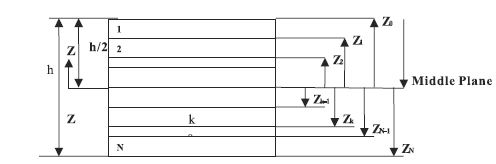
\includegraphics[scale=1.0]{figura/Stacking}
	\legend{Fonte: \cite{liu2004maximization}}
\end{figure}

Seguindo a metodologia para utilização dos parâmetros de laminação apresentada por \cite{miki1991optimum} e tendo como referência a \autoref{fig_stacking} considera-se uma sequência de laminação, em que cada lâmina é ortotrópica, como segue:

\begin{equation} \label{stacking}
[(\pm\theta_n)_{Nn}/\dots(\pm\theta_2)_{N2}/(\pm\theta_1)_{N1}]_s
\end{equation}

Segundo \cite{miki1991optimum}, os parâmetros de laminação são boas ferramentas para serem utilizadas como variáveis de projeto ao desenvolver um laminado, visto que é possível obter uma região viável dos parâmetros de laminação em um plano bidimensional. Quando tem-se um laminado simétrico e ortotrópico, a rigidez no plano (matriz A) e a rigidez flexural (matriz D) se tornam funções dos parâmetros de laminação, que são funções da sequência da laminação. E como este laminado é simétrico, a rigidez devido ao acoplamento no plano e a flexural (matriz B) é nula. Sabe-se que é possível através do método de utilizar parâmetros de laminação como variáveis de projeto, e obter pontos ótimos de projeto através de relações geométricas entre a região viável e a função objetivo do projeto.

Sabe-se, conforme demonstrado na seção da Teoria Clássica da Laminação, que:

\begin{equation} \label{ABD_definition}
\begin{gathered}
\begin{bmatrix}
    N \\
    M \\
\end{bmatrix}
=
\begin{bmatrix}
		A & B \\
		B & D \\
\end{bmatrix}
\begin{bmatrix}
    \varepsilon^o \\
    \kappa \\
\end{bmatrix}
\end{gathered}
\end{equation}

Segundo \cite{liu2004maximization}, as matrizes de rigidez A, B e D mostradas acima podem ser expressas em função dos invariantes de rigidez dos materiais $\emph{U}$ e de 12 parâmetros de laminação $\xi$ \cite{tsai1968invariant}. Considerando o laminado simétrico, a matriz de acoplamento de rigidez B será nula e então, o número de parâmetros de laminação será reduzido para 8. Considerando ainda, como prática de projeto adotada por vários fabricantes, que as lâminas são ortotrópicas e podem ter somente 0$^{\circ}$/$\pm$45$^{\circ}$/90$^{\circ}$ como ângulos de laminação, os parâmetros de laminação são reduzidos para 6. Tem-se, portanto, as seguintes expressões para a rigidez no plano e para a rigidez flexural:
\begin{equation} \label{A_matrix}
\begin{gathered}
\begin{bmatrix}
    A_{11} \\A_{12} \\A_{22} \\A_{66} \\A_{16} \\A_{26} \\
\end{bmatrix}
= h\begin{bmatrix}
		1 & \xi^A_1 & \xi^A_2 & 0 & 0 \\
		0 & 0 & -\xi^A_2 & 1 & 0 \\
    1 & -\xi^A_1 & \xi^A_2 & 0 & 0 \\
		0 & 0 & -\xi^A_2 & 0 & 1 \\
		0 & \frac{\xi^A_3}{2} & 0 & 0 & 0 \\
		0 & \frac{\xi^A_3}{2} & 0 & 0 & 0 \\
\end{bmatrix}
\begin{bmatrix}
    U_1\\U_2 \\U_3 \\U_4 \\U_5
\end{bmatrix}\\~\\
\begin{bmatrix}
    D_{11} \\D_{12} \\D_{22} \\D_{66} \\D_{16} \\D_{26} \\
\end{bmatrix}
= \frac{h^3}{12}
\begin{bmatrix}
		1 & \xi^D_1 & \xi^D_2 & 0 & 0 \\
		0 & 0 & -\xi^D_2 & 1 & 0 \\
    1 & -\xi^D_1 & \xi^D_2 & 0 & 0 \\
		0 & 0 & -\xi^D_2 & 0 & 1 \\
		0 & \frac{\xi^D_3}{2} & 0 & 0 & 0 \\
		0 & \frac{\xi^D_3}{2} & 0 & 0 & 0 \\
\end{bmatrix}
\begin{bmatrix}
    U_1\\  U_2 \\ U_3 \\ U_4 \\ U_5
\end{bmatrix}
\end{gathered}
\end{equation}

As propriedades de rigidez $\emph{Q}$ são dadas por:
\begin{equation} \label{Q_properties}
\begin{gathered}
Q_{11}=\frac{E_{11}}{1-\nu_{12}\nu_{21}}\\~\\
Q_{12}=\frac{\nu_{12}E_{22}}{1-\nu_{12}\nu_{21}}\\~\\
Q_{22}=\frac{E_{22}}{1-\nu_{12}\nu_{21}}\\~\\
Q_{21}=Q_{12}\\~\\
Q_{66}=G_{12}\\~\\
\nu_{21}=\nu_{12}\frac{E_{22}}{E_{11}}
\end{gathered}
\end{equation}\

E tem-se que os parâmetros de laminação relacionados ao plano $\xi^A_{[1, 2, 3]}$ e flexão $\xi^D_{[1, 2, 3]}$, são:
\begin{equation}\label{qsiA}
\begin{gathered}
	\xi^A_{[1, 2, 3]} = \frac{1}{h}\int^{\frac{h}{2}}_{\frac{-h}{2}}[\cos2\varphi, \cos4\varphi, \sin2\varphi]dz\\~\\
	\xi^D_{[1, 2, 3]} = \frac{12}{h^3}\int^{\frac{h}{2}}_{\frac{-h}{2}}[\cos2\varphi, \cos4\varphi, \sin2\varphi]z^2dz
\end{gathered}
\end{equation}\

Baseando-se nas equações \autoref{Q_properties} e \autoref{ABD_definition}, percebe-se que os parâmetros de laminação $\xi^D_3$ se relacionam com os termos $D_{16}$ e $D_{26}$ da matriz [D]. Estes termos não possuem uma contribuição significante para a análise e o critério de falha por flambagem que será avaliado, portanto, neste estudo o parâmetro $\xi^D_3$ será negligenciado. E como o laminado é simétrico e balanceado em relação ao plano médio o parâmetro de laminação $\xi^A_3$ também não será levado em consideração neste estudo, sobrando, portanto, os seguintes parâmetros de laminação que serão considerados durante a otimização do painel reforçado.
\begin{equation}\label{LP_AeD}
\begin{gathered}
\xi^A_{1} = \frac{1}{h}\int^{\frac{h}{2}}_{\frac{-h}{2}}[\cos2\varphi]dz\\~\\
\xi^A_{2} = \frac{1}{h}\int^{\frac{h}{2}}_{\frac{-h}{2}}[\cos4\varphi]dz\\~\\
\xi^D_{1} = \frac{12}{h^3}\int^{\frac{h}{2}}_{\frac{-h}{2}}[\cos2\varphi]z^2dz\\~\\
\xi^D_{2} = \frac{12}{h^3}\int^{\frac{h}{2}}_{\frac{-h}{2}}[\cos4\varphi]z^2dz
\end{gathered}
\end{equation}

Ainda que os parâmetros de laminação permitam uma otimização contínua do laminado com um número de variáveis de projeto relativamente baixo, eles não permitem a associação das restrições com a natureza discreta da espessura em ângulos de laminação \cite{liu2004maximization}. Por exemplo, com a utilização desse método não é possível prever a acomodação de várias lâminas em sequência com uma mesma direção de ângulo de laminação. Portanto, após a obtenção da otimização do laminado utilizando os parâmetros de laminação, será necessário recorrer a um banco de dados de laminados para obter a solução discreta do laminado.

Resumidamente, tem-se, portanto, que a relação, originalmente, não-linear entre a rigidez de um laminado e a sequência de laminação discreta se torna linear quando as funções trigonométricas são substituídas pelos parâmetros de laminação. Comparando-se à sequência de laminação discreta, os parâmetros de laminação podem ser utilizados como variáveis contínuas e adimensionais dentro de uma otimização baseada no gradiente, conforme abordado nas seções seguintes.

%\subsection{Soma dos parâmetros de laminação}
%(ESCREVER SOBRE)

\section{Práticas de projeto adotadas}
Esta seção apresenta regras e práticas relevantes utilizadas durante o projeto de estruturas em materiais compostos na indústria aeronáutica.

\subsection{Laminados simétricos}
Os laminados que possuem um sequência	de ângulos das lâminas simétrico em relação ao plano médio, são chamados de laminados simétricos. Conforme descrito por \cite{mil2002handbook} e \cite{niucomposite}, a maior vantagem da utilização de um laminado simétrico é o desacoplamento entre o comportamento de membrana e flexão da estrutura.

Em um laminado simétrico, conforme notação apresentada na \autoref{fig_laminate} e conforme a \autoref{eq_matrixB} matriz [B] do laminado se anula.

\begin{figure}[h]
	\caption{\label{fig_laminate}Notação para espessura do laminado e sequência das lâminas}
  \centering
  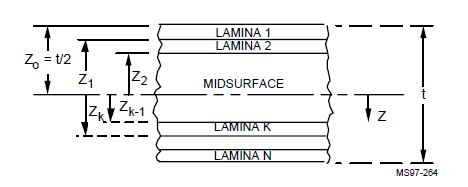
\includegraphics[scale=1.0]{figura/Laminate}
	\legend{Fonte: \cite{mil2002handbook}}
\end{figure}

\begin{equation} \label{eq_matrixB}
B_{ij}
=
\sum_{k=1}^N (\overline{Q}_{ij})_k [z_k^2 - (z_{k-1})^2]
\end{equation}

Sabe- se que $ \overline{Q}_{ij} $ corresponde a rigidez da lâmina. E sabe-se também que a matriz $ B_{ij} $ é a responsável pelo acomplamento entre a reposta no plano e a flexão do laminado. Portanto, conforme \cite{nasa1997guidelines}, quando a matriz $ B_{ij} $ não é zerada, um carregamento no plano induz curvaturas, e momentos de flexão induzem deformações no plano. Nota-se pela \autoref{eq_matrixB} que a matriz $ B_{ij} $ possui termos da coordenada z elevados ao quadrado, portanto, quando o laminado possui simetria geométrica e de materiais em relação ao plano médio, este termo é zerado, e portanto, tem-se $ B_{ij} = 0$.

\subsection{Laminados balanceados}
Os laminados balanceados são aqueles em que todas as lâminas, com exceção das de 0$^{\circ}$ e das de 90$^{\circ}$, devem ocorrer em pares de $ +\theta $ e $ -\theta $ acima e abaixo do plano médio do laminado. Para o conjunto de laminados compostos por lâminas com ângulos 0/$\pm$45/90, cada lâmina de +45$^{\circ}$ deve ser acompanhada de um lâmina de -45$^{\circ}$.
Laminados balanceados possuem vantagens similares às vantagens do laminados simétricos. Uma delas é que o acoplamento de membrana entre o comportamento normal e de cisalhamento no plano da estrutura é removido, visto que ambos os coeficientes, $ A_{16} $ e $ A_{26} $, são iguais a zero \cite{nasa1997guidelines}. Este comportamento pode ser explicado observado as equações do carregamento de membrana de um laminado simétrico, \autoref{eq_loadingA}, \autoref{eq_A16} e \autoref{eq_A26}.

\begin{equation} \label{eq_loadingA}
\begin{bmatrix}
    N_{x} \\
    N_{y} \\
    N_{xy} \\
\end{bmatrix}
=
\begin{bmatrix}
    A_{11} & A_{12} & A_{16}\\
    A_{12} & A_{22} & A_{26}\\
    A_{16} & A_{26} & A_{66}\\
\end{bmatrix}
\begin{bmatrix}
    \varepsilon_{x}^o \\
    \varepsilon_{y}^o \\
    \gamma_{xy}^o \\
\end{bmatrix}
\end{equation}

\begin{equation} \label{eq_A16}
A_{16}
=
\sum_{k=1}^N (\overline{Q}_{16})_k t_k
\end{equation}

\begin{equation} \label{eq_A26}
A_{26}
=
\sum_{k=1}^N (\overline{Q}_{26})_k t_k
\end{equation}

Onde

\begin{equation} \label{eq_Q16}
(\overline{Q}_{16})_k
=
({Q}_{11}-{Q}_{12}-2{Q}_{66})_k \sin\theta \cos^3\theta + ({Q}_{11}-{Q}_{22}-2{Q}_{66})_k \sin^3\theta \cos\theta
\end{equation}
\begin{equation} \label{eq_Q26}
(\overline{Q}_{26})_k
=
({Q}_{11}-{Q}_{12}-2{Q}_{66})_k \sin^3\theta \cos\theta + ({Q}_{11}-{Q}_{22}-2{Q}_{66})_k \sin\theta \cos^3\theta
\end{equation}

Sabe- se que $ \overline{Q}_{ij} $ corresponde a rigidez da lâmina e que $ t_k $ corresponde a espessura da lâmina. Nota-se também que ambas as expressões de $ A_{16} $ e $ A_{26} $ contém potências ímpares de $ \sin\theta $ e $ \cos\theta $. Logo lâminas com ângulos de 0$^{\circ}$ e 90$^{\circ}$ não contribuem para os termos de $ A_{16} $ e $ A_{26} $ e estes termos são reduzidos a zero em qualquer laminado balanceado \cite{nasa1997guidelines}.

A \autoref{fig_balancedlaminate} apresenta dois laminados, um desbalanceado, visto que faltam lâminas com -45$^{\circ}$ e um balanceado.

\begin{figure}[ht]
	\caption{\label{fig_balancedlaminate}Laminado desbalanceado e laminado balanceado}
  \centering
  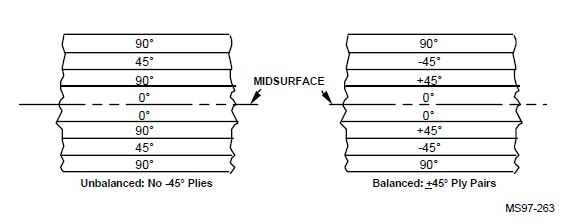
\includegraphics[scale=1.0]{figura/BalancedLaminate}
	\legend{Fonte: \cite{mil2002handbook}}
\end{figure}

Portanto, satisfazendo esta prática de projeto de utilizar somente laminados balanceados, tem-se a seguinte \autoref{eq_result_loadingA} resultante para tensão-deformação

\begin{equation} \label{eq_result_loadingA}
\begin{bmatrix}
    N_{x} \\
    N_{y} \\
    N_{xy} \\
\end{bmatrix}
=
\begin{bmatrix}
    A_{11} & A_{12} & 0\\
    A_{12} & A_{22} & 0\\
    0 & 0 & A_{66}\\
\end{bmatrix}
\begin{bmatrix}
    \varepsilon_{x}^o \\
    \varepsilon_{y}^o \\
    \gamma_{xy}^o \\
\end{bmatrix}
\end{equation}

\subsection{Regra dos 10\%}
Esta prática de projeto não é determinada por documentação  para ser rigorosamente seguida e também não há nenhuma documentação formal que comprove a sua validade. No entanto, esta prática foi seguida por diversas campanhas de projetos de estruturas em materiais compostos e demonstrou bons resultados e portanto, é adotada até os dias atuais em diversos programas. A regra dos 10\% determina que cada ângulo de laminação (0$^{\circ}$,$\pm$45$^{\circ}$ e 90$^{\circ}$) compreenda em pelo menos 10\% das camadas do laminado final. O uso desta prática de projeto conduz a laminados utilizáveis que são mais robustos pelo fato de que eles menos susceptíveis à fragilidade associada aos laminados rigorosamente ortotrópicos \cite{nasa1997guidelines}.

Além disso, segundo \cite{mil2002handbook}, um comportamento do laminado dominado pela matriz, ou seja, efeitos não lineares, pode ser evitados em laminados onde a direção principal da fibra não é alinhada com o eixo principal do carregamento.
